%=========================================================================
% fig-opts-avx-vec.tex
%=========================================================================

\begin{figure}

  \centering
  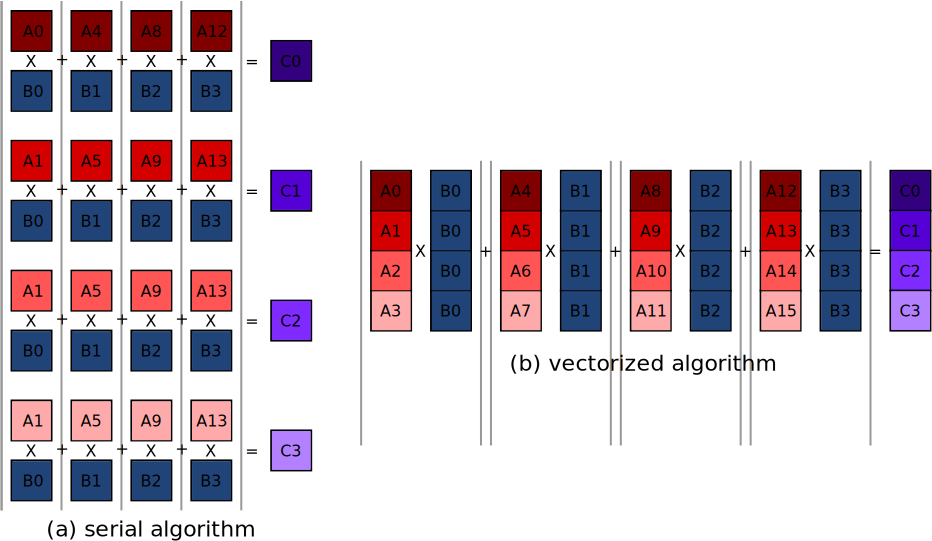
\includegraphics[width=\tw]{fig-opts-avx-vec.svg.pdf}

  \caption{\textbf{Overview of Vectorization Strategy --} For simplicity,
    4x4 matrices are shown with elements labeled in the column-major
    order. The computation required to generate the elements of a single
    column of the output matrix can be re-arranged to group multiple
    elements of the input matrix into a vector register. This effectively
    allows us to compute multiple elements of the output matrix in
    parallel (i.e., 4 doubles in parallel with 256b SIMD pipeline).}

  \label{fig-opts-avx-vec}

\end{figure}
